%%%%%%%%%%%%%%%%%%%%%%%%%%%%%%%%%%%%%%%%%%%%%%%%%%%%%%%%%%%
\documentclass[letterpaper, 12 pt]{article} 

\usepackage[a4paper,left=2cm,right=2cm,top=3cm,bottom=3cm]{geometry}
\usepackage{float, graphicx} % Images.
\usepackage{multicol}
\usepackage{times}
\usepackage{lipsum}

\parindent 0pt

\title{\Large \bf VODOM - Monocular Visual Odometry Pipeline}

\author{
  Nikhilesh Alatur\\\texttt{14-934-004}
  \and
  Simon Schaefer\\\texttt{14-943-799}
}
\date{\vspace{-3ex}}

\begin{document}
\maketitle

\begin{multicols*}{2}
\section{Problem}
The goal of this mini-project is to implement a simple, calibrated, monocular, visual odometry (VO) pipeline with the most essential features: initialization of 3D landmarks, keypoint tracking between two frames, pose estimation using established 2D - 3D correspondences and triangulation of new landmarks. The algorithm is implemented in \textsc{Matlab}(Version R2018a) and tested on several datasets, such as KITTI, Malaga, a parking garage and a self-recorded dataset at ETH. 

\section{Conventions}
Pose transformations between frames $A$ and $B$ are denoted with rotation matrix and translation vector $R_{AB}$ and $t_{AB}$ such that the origin of $B$ expressed in $A$ is at $t_{AB}$ and the $(x,y,z)$ unit vectors of frame $B$ expressed in frame $A$ are the columns of $R_{AB}$.The frame $W$ denotes the world frame and $C$ the camera frame. In the datasets used the camera looks in positive $z$ direction, $x$ points to the right and $y$ down in the image, such that we are mainly interested in the $x-z$-plane. We assume that the 0th camera frame coincides with the world frame.

\section{Approach}
\subsection{Overview}
The underlying visual odometry pipeline is based on the Markov assumption, i.e. the current and previous input as well as merely the previous state are sufficient to determine the current state. Thereby, a state contains the following variables: 

\begin{itemize}
\item $X$: Valid landmarks as positions in homogeneous coordinates w.r.t. world frame [$4\times M$ matrix]
\item $P$: Valid keypoints as pixel coordinates in current image frame [$2 \times M$ matrix]
\item $P_{cand}$: Possible keypoints, which we might use for triangulating new landmarks, as pixel coordinates in current image frame [$2 \times L$ matrix]
\item $P_{cand}^{orig}$: Pixel location, when the candidate keypoints was initially found [$2 \times L$ matrix]
\item $T_{cand}^{orig}$: Camera pose at the time when the candidate keypoints was initially found [$16 \times L$ matrix]
\item $c$: Counter array for valid 2D-3D-correspondences [$M \times 1$ vector]
\item $c_{cand}$: Counter array for candidate keypoints [$L \times 1$ vector]
\item $T_{WC}$: Homogeneous transformation matrix from world to camera frame w.r.t. world frame as $4 \times 4$ matrix
\end{itemize}

\begin{figure}[H]
\begin{center}
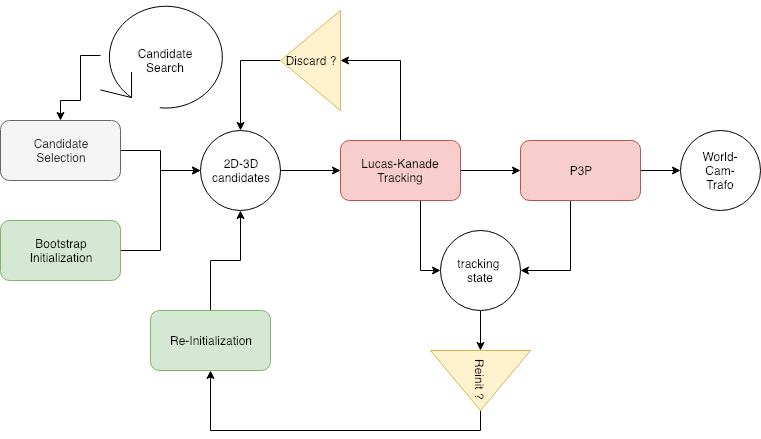
\includegraphics[width=\linewidth]{process.png}
\end{center}
\caption{Pipeline - Flowchart}
\label{fig:process}
\end{figure}

In general, the transformation from one to another frame is estimated, by either tracking or matching keypoints, determining 2D-3D correspondences and triangulating the transformation. As shown in Fig. \ref{fig:process} initially keypoint matching (harris features and patch matching) is used to generate an initial set of keypoints and to triangulate an initial poincloud. Afterwards, in continuous operation, the keypoints are tracked using KLT, while new (valid) 2D-3D correspondences are derived using a candidate selection algorithm. Using the valid 2D-3D correspondences the transformation between the frames is estimated using RANSAC-supported P3P. 

\subsubsection{\textit{Note}}
\textit{Within the report the underlying algorithm mainly is described in general, since most of parameters are dataset specific. The exact parameters can be looked up in the parameter file of the implementation. }

\subsubsection{Why not Feature Matching only ?}
Instead of the combination of feature matching and tracking it is possible to merely use feature matching between subsequent frames in order to estimate the camera's pose. As shown for an examplic curve in the KITTI dataset in Fig. \ref{fig:matching_only} this approach already leads to reasonable results. 

\begin{figure}[H]
\begin{center}
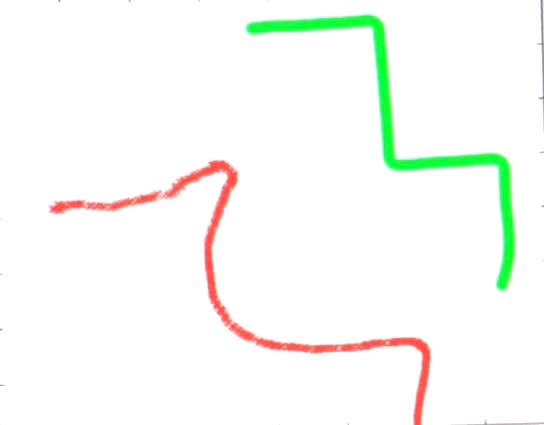
\includegraphics[width=4cm]{matching_only.jpeg}
\end{center}
\caption{Matching Only Approach (green = ground truth, red = matching only estimate)}
\label{fig:matching_only}
\end{figure}

However, KLT turned out to be faster, more resistant to outlier and yielding less mismatches. However, continuously tracking leads to a lot of drifting in scale while the scale in feature matching can be adapted. Therefore, the combination (tracking AND occasionally feature matching, i.e. re-initialization) performs best. 

\subsection{Bootstrap Initialization}
The goal of bootstrap initialization is to find an accurate  initial set of landmarks $X$ and their keypoint correspondences $P$. To do so feature matching is applied between two initial images $I_{b0}$ and $I_{b1}$, using Harris (corners) features and simple patch descriptors (quadratic patches with size $= (2*r + 1)^2$, $r_p = r_d = 9$). Based on the keypoint matches the transformation between both frames is found by first computing the fundamental matrix in a RANSAC approach. Here we sample multiple times 8 matches, compute the fundamental matrix with the 8-point algorithm and then check for inliers. We then select the fundamental matrix $F$ with the most inliers as the real fundamental matrix, relating both views Now, we can easily extract the essential matrix $E$, as we have access to the camera's intrinsics $K$. Then we disambiguate the four possible transformations that can be extracted from the essential matrix, by triangulating landmarks and selecting the one solution where we get the most landmarks in front of our cameras. Finally we get the homogenous transformation between the bootstrap frames and also an initial set of keypoints and the corresponding 3D landmarks.

\subsubsection{Baseline}
In determining the baseline, e.g how many frames the bootstrap images lie apart, a trade-off has to be made between finding a lot of matches ($I_{b0}$ and $I_{b1}$ close) and minimizing the depth error by increasing the baseline ($I_{b1}$ far away from $I_{b0}$). This trade-off is specific for each dataset. Furthermore, sometimes we couldn't take the first image in the dataset as bootstrap image, as it had too little texture (e.g in the parking dataset). In such cases we took the first image, where had a reasonable amount of texture (e.g frame 10 in parking dataset).

\subsubsection{Patch size}
Both the corner detection as well as the patch description are implemented using a patch size of $9$. Larger patch sizes were tested but they only slowed down the pipeline without significantly improving the results. 

\subsubsection{Matching Lambda}

\begin{figure}[H]
\begin{center}
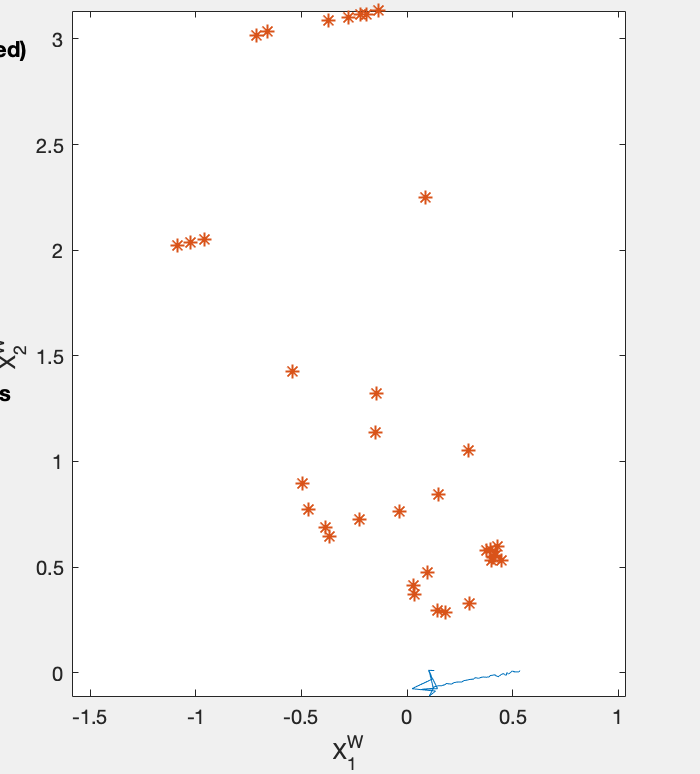
\includegraphics[height=3.5cm]{matching_lambda_bad.png}
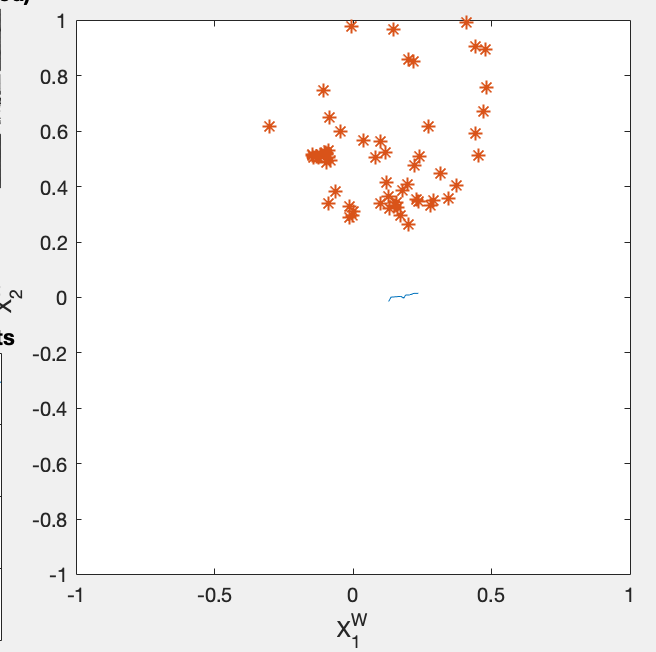
\includegraphics[height=3.5cm]{matching_lambda_good.png}
\end{center}
\caption{Feature matching - Effect of $\lambda$ (left: $\lambda = 10$, right: $\lambda = 5$). Worse initial transformation in case of larger $\lambda$ (parking dataset).}
\label{fig:matching_lambda}
\end{figure}

To match the feature, we look for matches where the SSD between the descriptors of each possible feature pair is minimized. The closeness of being a match is determined by $\lambda$ (in relative to smallest SSD value), Fig. \ref{fig:matching_lambda} displays the effect of the $\lambda$ on the final point cloud and motion estimate. A large $\lambda$ lets pass a lot of eventual matches which results in more landmarks to track later on but also in a worse initial point cloud (comp. $\lambda = 10$, unrealistic motion, in comparison to $\lambda = 5$), another dataset specific trade-off.

\subsubsection{Fundamental Matrix Estimation - RANSAC Trials}
In theory, 8 inliers are required to run the 8 point algorithm, therefore the number of searching iterations has to trade-off performance and the chance to find a  sufficient number of "close" inliers, $200$ iterations are optimal here. However, although outlier rejection is applied (real) outliers still can be regarded as inliers, e.g. in case of mismatches or just due to randomness, which can lead to "wrong" transformations.
\newline 
During implementation we decided to not use the Matlab function \textit{estimateFundamentalMatrix}, but to implement the RANSAC-based fundamental matrix estimation by our own, as we faced severe issues regarding both the minimal number of input matches (which seems to have to be way larger than the theoretical 8 matches) as well as the number of resulting inliers (whereby next to LMedS also other methods have been tried). 

\subsection{Continuous Operation}
Given the initial set of 2D-3D correspondences to estimate the transformation between $I_i$ and $I_{i-1}$ for $i > b_1$ the Lucas-Kanade Tracking (KLT) and the P3P algorithm are used. However, the inital set of correspondences will eventually get out of view so that we have to take care of having always enough features before running out of sufficient matches. Therefore, in every frame new keypoints are extracted which are possible valid keypoints, to be used later for triangulating new landmarks (candidate search), while previously extracted candidates are transformed to valid keypoints (candidate selection). Nevertheless in some cases the generation of valid correspondences by candidate selection is not sufficient to ensure a reasonable number of 2D-3D correspondences to base the P3P pose estimate on. Therefore, re-initialization is necessary forcing the search for new (valid) keypoints and landmarks by using a similar approach as in the bootstrap.

\subsubsection{KLT}
For KLT the Matlab vision toolbox (function: \textit{vision.PointTracker}) is utilized, accepting every tracked pixel by allowing a bidirectional error. To be able to select candidates to be "valid" keypoints later on, next to the "valid" keypoints also all of the candidate keypoints are tracked. 
\newline
The bidirectional error implies another trade-off similar to the $\lambda$-trade-off above, accepting more keypoint matches to reason the pose estimate on more keypoints or merely accept comparable "good" trackings. However, the algorithm turned out to be more reliable allowing infinite bidirectional tracking error for mainly two reasons. First, accepting less matches can result in re-initialization (as shown later on) introducing more outliers than continuing tracking and second, the pose estimate involves RANSAC so that "bad" matches probably won't be taken into account anyway. 

\begin{figure}[H]
\begin{center}
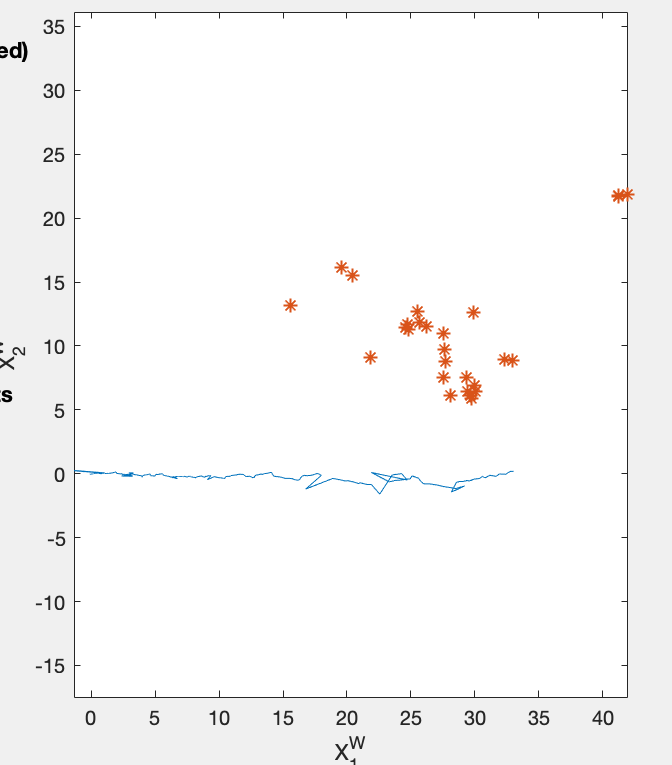
\includegraphics[height=3.5cm]{parking_100bi.png}
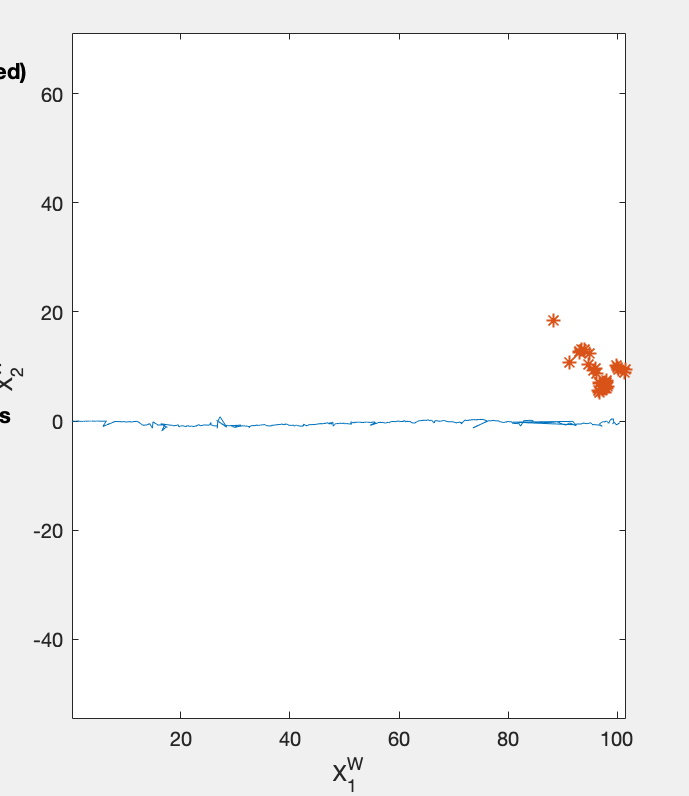
\includegraphics[height=3.5cm]{parking_infbi.png}
\end{center}
\caption{KLT - Effect of bidirectional error (left: $be = 100$, right: $be = \infty$). More inaccurate motion estimates (blue line) in case of smaller allowed bidirectional error  (parking dataset).}
\label{fig:klt_error}
\end{figure}

\subsubsection{P3P}
The P3P algorithm requires 3 points to calculate the pose out of known correspondences of landmarks positions and pixel coordinates. However, even the correspondences which have been selected as being "valid" suffer from outliers, so that P3P cannot be applied directly. Instead RANSAC is applied for outlier rejection, iteratively choosing samples of 3 correspondences and finding the most probable pose which has the largest count of reprojection inliers (allowing a tolerance of 5 pixels error). The P3P outliers are discarded since they do not reflect the current pose estimate anymore. For the final pose estimate the transformation matrix of the best RANSAC iteration is used (not DLT !). 
\newline
For P3P the reprojection error turned out to be very important, since small reprojection error ensures a better transformation estimate but, in general, also requires more correspondences and more RANSAC iterations and therefore rather leads to re-initialization (drift !). 
\newline 
As for the fundamental matrix estimate the number of RANSAC iterations is an important parameter, trading performance against accuracy. Although in theory P3P requires 3 points to find "good" inliers reliably many more iterations are necessary, ending up in 200 iterations (although around 80 iterations are sufficient in most cases). 
\newline
As for the fundamental matrix estimation for P3P the Matlab implementation (function: \textit{estimateWorldCameraPose}) has been tried but met similar problems so that we decided to implement the RANSAC algorithm manually. 

\subsubsection{Candidate Selection}
As already mentioned, at one point KLT will loose the keypoints, as KLT only does tracking. For this we continuously find new keypoints, which we might use at a later point if it becomes necessary, for updating our landmarks pointcloud. After we have done P3P and found our most recent camera transformation, we look for new landmarks. For this purpose, we take all candidate keypoints, which satisfy some heuristics. First of all, the candidate keypoints must have been detected in a frame not later than three frames before the current frame and they must not have been detected in a frame, that is further away than 10 frames from our current frame. This ensures that the baseline is big enough for triangulating the landmark and also ensures that we don't have wrong matches, as the longer the baseline the less likely the match can be correct (it's unreasonable that the same feature can be seen in so many frames). The selected keypoint are then triangulated and accepted if they pass some basic sanity checks. For example they have to lie in front of the camera and their depth mustn't exceed a limit, as this might be an indication for a big depth error. Finally the chosen keypoints are deleted from the list of candidate keypoints, such that they are not checked again in the next frames.

\subsubsection{Candidate Search}
For continuously adding possible "valid" keypoints candidates are search for in every iteration, using Harris corner detection. Here, to avoid non-unique keypoints a new candidate has to be located in a minimal distance (or further away) from already existing keypoints. As the camera does not move a lot from one frame to another a small number of newly added candidates is sufficing compared to the number of detected features while bootstrap initialization. Also a small number ensures to merely choose features having a high Harris scores and therefore are easier to re-find and track (large gradients !). The number of newly detected features largely depends on the dataset, while quite small for KITTI it should be quite large for parking and Malaga (being counter-proportional to the minimal distance). 

\subsubsection{Post-Processing}
All of the previously mentioned steps might lead to invalid correspondences, e.g. when KLT cannot track "valid" keypoints anymore or when they are outliers in the P3P pose estimate.If they would be continued as "valid" correspondences they would possibly corrupt the pose estimates in the following iterations. Therefore, they are removed in post-processing. To do so the counter $c$ (comp. state) is set to nonzero values everytime a correspondence fails. 
\newline
Similarly, candidate keypoints are removed in post-processing. Additionally, the candidates are punished for not being selected as "valid" keypoints in subsequent iterations and removed after 11 punishments. 

\subsubsection{Re-Initialization}
Despite of the ongoing update of "valid" correspondences there might not be a sufficiently large amount of correspondences to continue tracking and using P3P reliably. In this cases a re-initialization is necessary. 
\newline
Re-Initialization involves feature matching and a pose estimate based on a RANSAC-supported fundamental matrix estimation similar to bootstrap initialization. Additionally, candidate search is applied to prevent another re-initialization procedure within the next few iterations. While the scale retained automatically while tracking in re-initialization it is unknown a priori and has to be determined such that it matches the previously used scale. Therefore, the translation vector is assumed to be roughly constant in magnitude (norm) over the last frames. Following this assumption the scale is determined by computing the norm of the translation vector over the previous frames by deriving the transformation from the fifth last frame $I-5$ and the last frame $I-1$

$$T_{CcCp} = T_{I-1W}^{-1} T_{I-5W}$$

assuming re-initialization between the current and the fourth last frame $I-4$. Balancing the baseline for re-initialization ($4$ frames in the given example) between scale drift (more for larger baseline) and depth error (less for larger baseline) is another trade-off.  

\subsection{Groundtruth Alignment}
After running the visual odometry on the whole dataset the estimated trajectory is compared to the groundtruth (if available). Since the pipeline can estimate the trajectory up to a scale factor and to deal with errors in the initial rotation estimate, bundle adjustment is applied finding the scale and initial rotation minimizing the overall SSD between trajectory and groundtruth (no optimization !). 

\subsection{Visualization}
In every iteration of continuous operation the tracked keypoints, number of candidates and "valid" correspondences as well as the landmarks and estimated poses are visualized, as shown in Fig. 

\begin{figure}[H]
\begin{center}
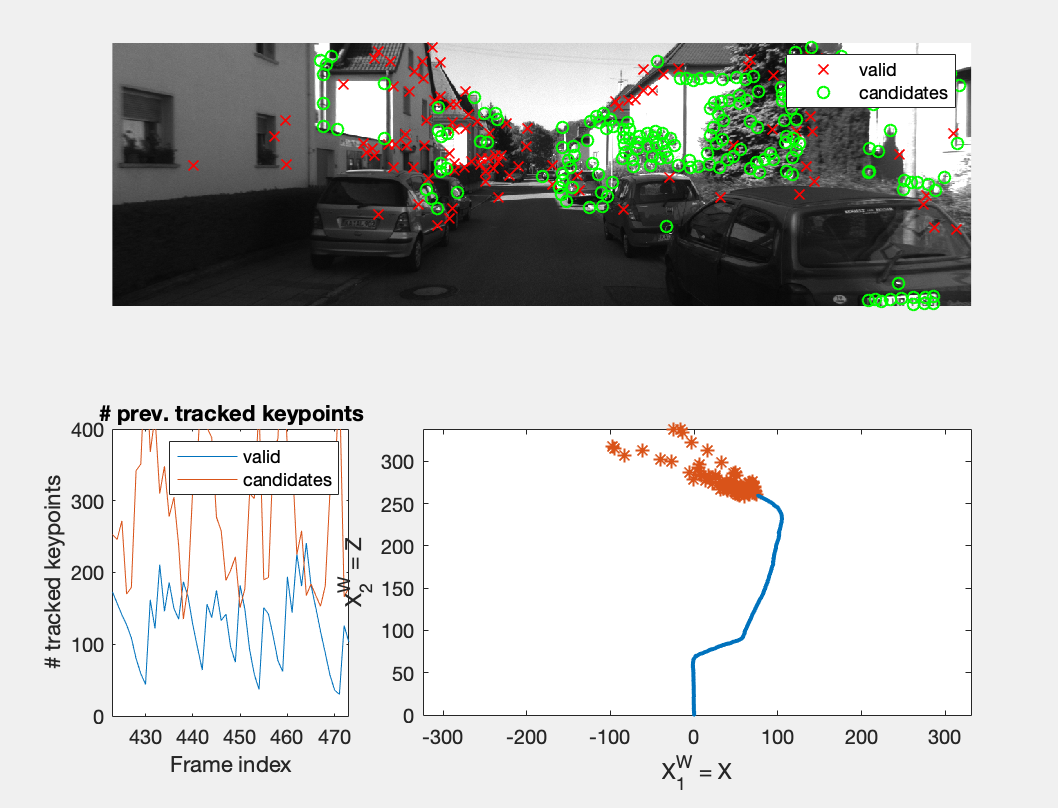
\includegraphics[width=\linewidth]{visualisation.png}
\end{center}
\caption{Pipeline - Visualization}
\label{fig:visualisation}
\end{figure}

\section{Results}
In the following the results of the purposed algorithm are shown w.r.t. several datasets. Thereby, the green line represents the ground-truth while the blue line shows the computed trajectory. In general the visual odometry pipeline works and has reasonable performance in both accuracy (as shown in detail below) and speed. Nevertheless, especially in long-term it is quite vulnerable to small errors in rotation estimation, as not perfectly optimized and only mono-vision based. 

\subsection{KITTI}
The algorithm was developed mainly using the KITTI dataset and therefore performs quite well on this dataset. It can perfectly handle both the features very far away (good for rotation estimation) and close the optical axis as well as the close features (good for translation estimation) at the side. Nevertheless, while smooth curves can be dealt with reasonably the sharp curves can lead to rotation error (as shown in Fig. \ref{fig:results_kitti}). 

\begin{figure}[H]
\begin{center}
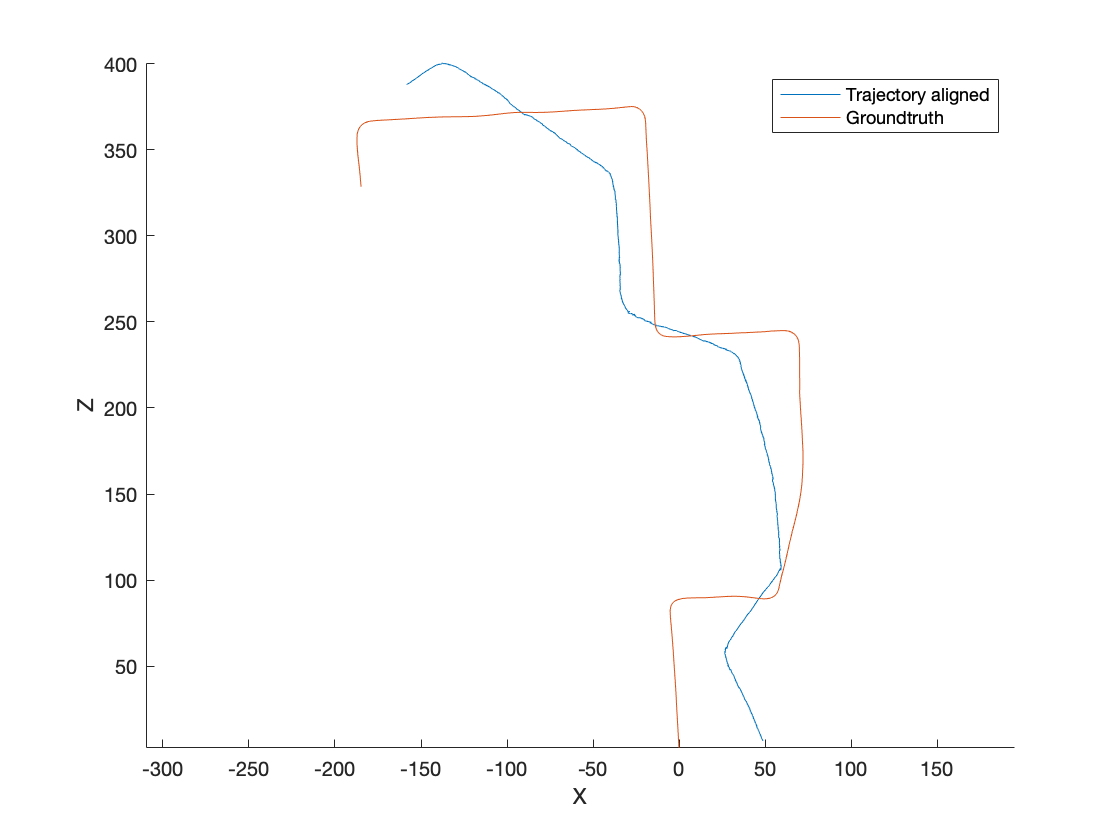
\includegraphics[width=\linewidth]{kitti.png}
\end{center}
\caption{KITTI dataset - Resulting trajectory vs Groundtruth}
\label{fig:results_kitti}
\end{figure}

Anyways, as no bundle adjustment is applied, due to drift and rotation inaccuracies in global scale (i.e. the whole dataset) the estimated trajectory drifts apart. 

\subsection{Malaga}
The malaga dataset is quite close to the KITTI dataset, as it contains images taken by a camera attached to a car driving through city area, but has less sharp curves. Features like the edges of the centre strip are very useful as they are close and distinct and for this reason often selected as "valid" correspondence. These features are however lost faster compared to features in the horizon so that the amount of candidates to be detected in each frame needs to be larger, in order to ensure a continuous tracking procedure. 

\begin{figure}[H]
\begin{center}
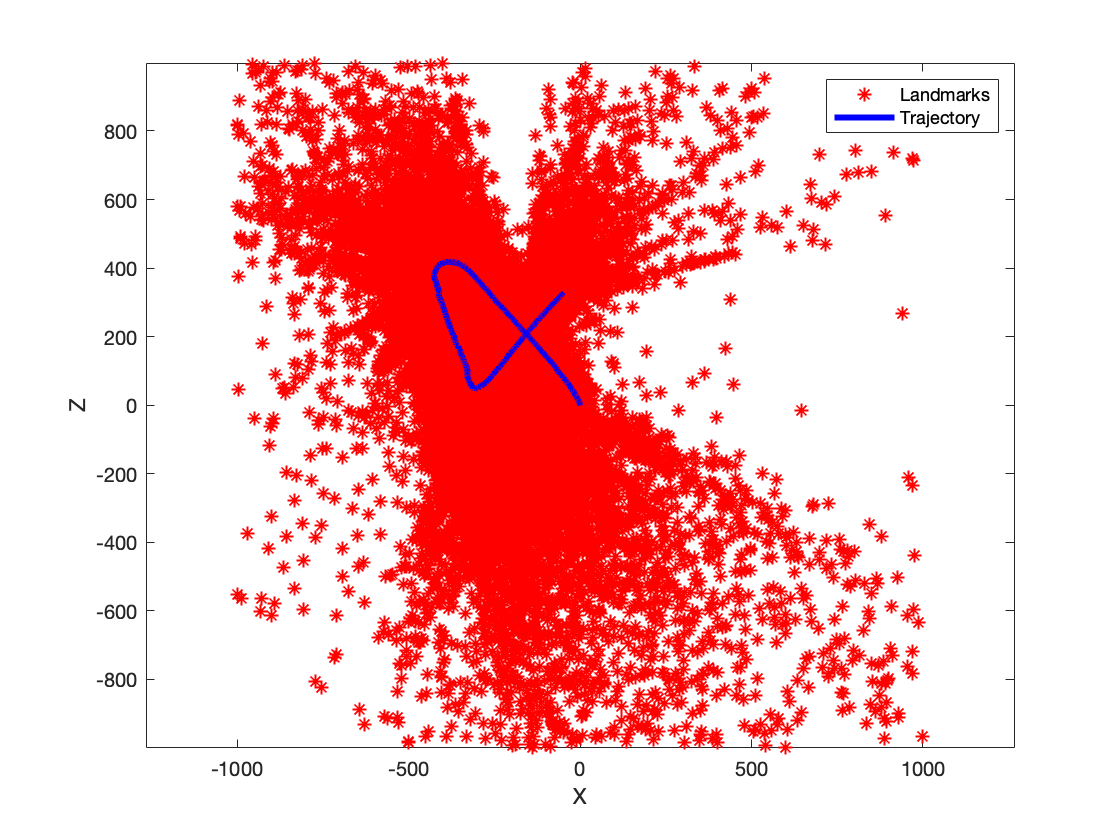
\includegraphics[width=\linewidth]{malaga.png}
\end{center}
\caption{Malaga dataset - Resulting trajectory vs Groundtruth}
\label{fig:results_malaga}
\end{figure}

\subsection{Parking}

\begin{figure}[H]
\begin{center}
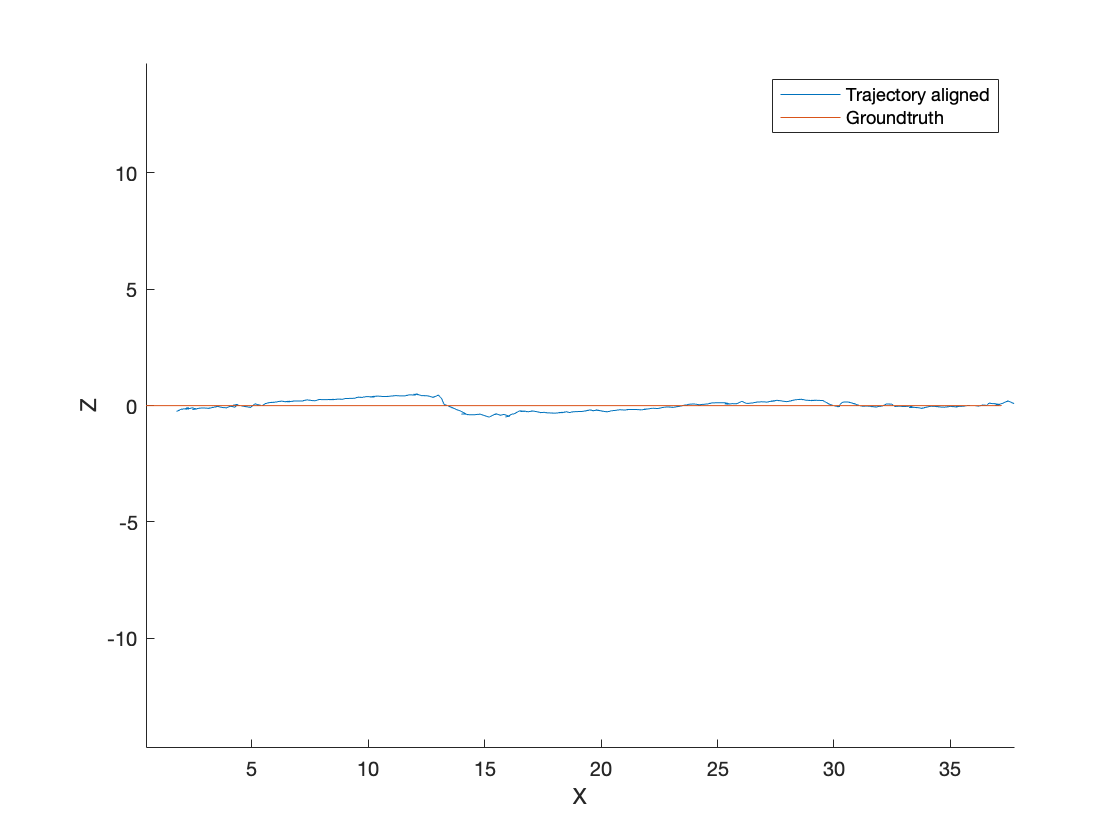
\includegraphics[width=\linewidth]{parking.png}
\end{center}
\caption{Parking dataset - Resulting trajectory vs Groundtruth}
\label{fig:results_parking}
\end{figure}

The parking dataset has continuous movement in $x$-direction, therefore small miscalculations in rotation have a large effect. As shown in Fig. \ref{fig:results_parking} the ground truth can be tracked reasonably accurate, despite of small rotation errors. Besides, in parking dataset we faced the problem of either untracked or outlier correspondences in certain regions (as the landmarks are pretty far away), such that in order to preserve a reasonable amount of "valid" correspondences, the number of extracted candidates and the matching threshold are chosen very large.

\subsection{ETH}
Next to the standard datasets mentioned above we recorded two additional datasets at ETH. \textit{ETH Long} has roughly 1000 frames and very sharp curves (nearly pure rotation). Using a much higher rate of re-initialization as shown in Fig. \ref{fig:results_eth_long} our algorithm can handle these sharpe turns (note: the datasets are recorded by centimeter scale movements, the "jiggling" trajectory estimate in real scale therefore is less than a few centimeters inaccuracy).

\begin{figure}[H]
\begin{center}
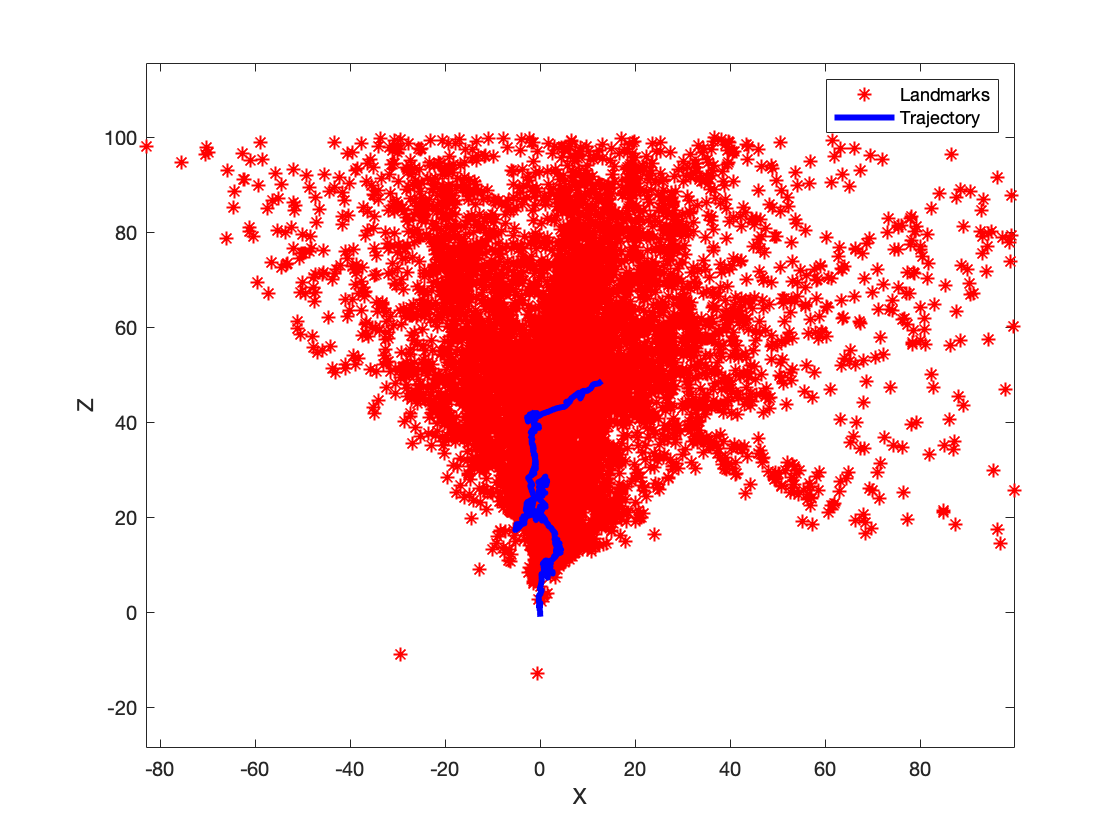
\includegraphics[width=\linewidth]{eth_long.png}
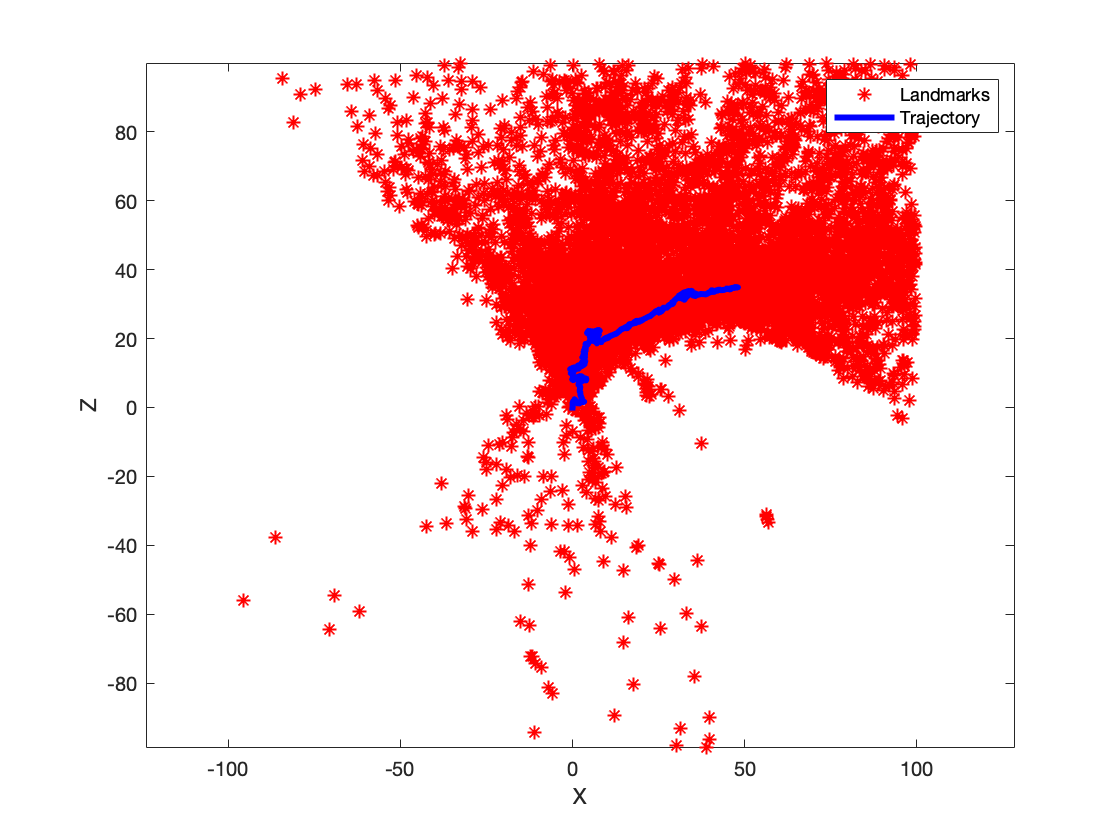
\includegraphics[width=\linewidth]{eth_long2.png}
\end{center}
\caption{ETH long dataset - Resulting trajectory vs Groundtruth}
\label{fig:results_eth_long}
\end{figure}

 For the \textit{ETH April} dataset we used an april tag localization algorithm (wiki.ros.org/apriltags\_ros) to estimate a position ground truth. Our VO algorithm also succeeds in this dataset. Since both dataset's images are comparably small ($480\times 640$ resolution) a lot less keypoint correspondences have to be used. 

\begin{figure}[H]
\begin{center}
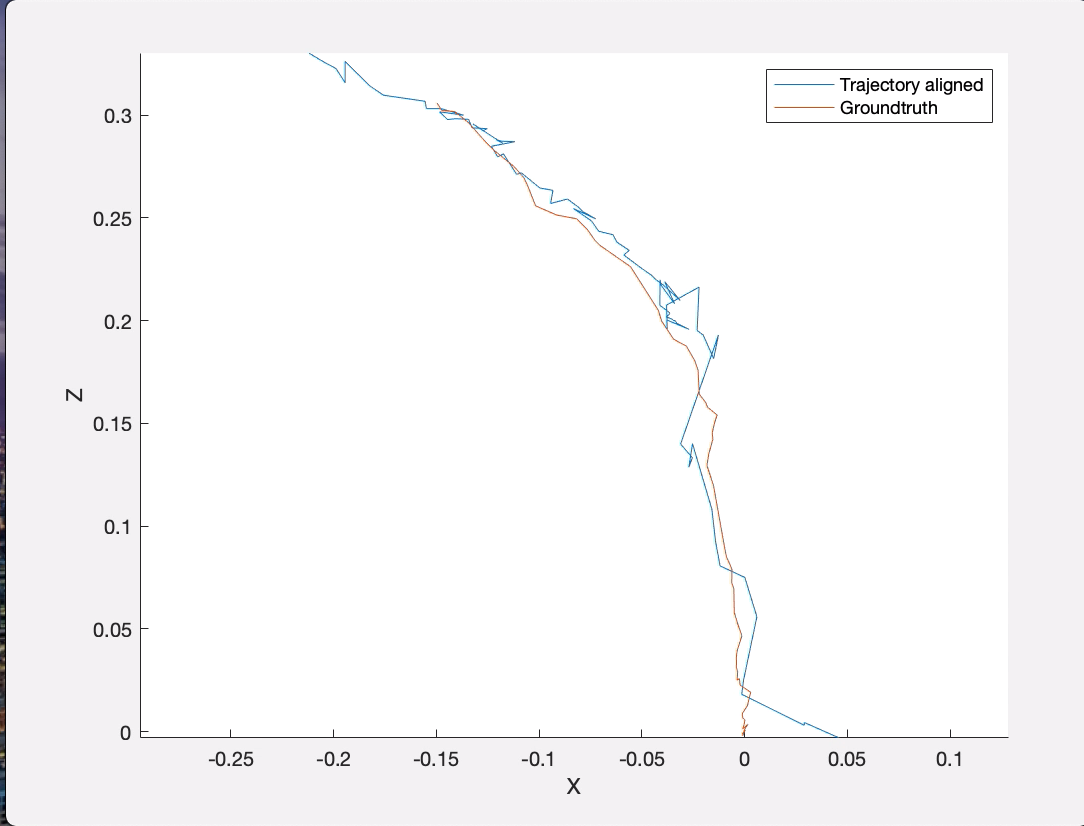
\includegraphics[width=\linewidth]{eth_april.png}
\end{center}
\caption{ETH april dataset - Resulting trajectory vs Groundtruth}
\label{fig:results_eth_april}
\end{figure}

\section{Further Development}
Although the basic framework is working further parameter tuning can still improve the results a lot, especially in terms of rotational accuracy of the pose estimate (e.g. in curves). 
Besides, as further development an inertial unit can be integrated in order to increase outlier reliability and decrease drift, as does an online (window-based) bundle adjustment. Furthermore, although it was not in the project's scope, the implemented visual odometry pipeline is quite slow (2-3 frames per second) and therefore far away from real time. Code optimization, parameter tuning, parallelization of RANSAC (etc.) and a migration to a more performant programming environment  (e.g. C++) would boost the performance. 

\end{multicols*}
\end{document}